\documentclass[aps,prl,twocolumn,superscriptaddress]{revtex4-1}
% \documentclass[aps,twocolumn,secnumarabic,balancelastpage,amsmath,amssymb,nofootinbib]{revtex4-1}
\usepackage{amsmath}
\usepackage{amssymb}
\usepackage{amsfonts}
\usepackage{color}
\usepackage{graphics}
\usepackage[pdftex]{graphicx}
\usepackage[utf8x]{inputenc}
\usepackage[colorlinks=true]{hyperref}
\usepackage{footmisc}
\usepackage{braket}

\newcommand{\ud}{\mathrm{d}}
\newcommand{\ue}{\mathrm{e}}
\newcommand{\ui}{\mathrm{i}}
\newcommand{\res}{\mathrm{Res}}
\newcommand{\Tr}{\mathrm{Tr}}
\newcommand{\dsum}{\displaystyle\sum}
\newcommand{\dprod}{\displaystyle\prod}
\newcommand{\dlim}{\displaystyle\lim}
\newcommand{\dint}{\displaystyle\int}
\newcommand{\fsno}[1]{{\!\not\!{#1}}}
\newcommand{\texp}[2]{\ensuremath{{#1}\times10^{#2}}}
\newcommand{\dexp}[2]{\ensuremath{{#1}\cdot10^{#2}}}
\newcommand{\eval}[2]{{\left.{#1}\right|_{#2}}}
\newcommand{\paren}[1]{{\left({#1}\right)}}
\newcommand{\lparen}[1]{{\left({#1}\right.}}
\newcommand{\rparen}[1]{{\left.{#1}\right)}}
\newcommand{\abs}[1]{{\left|{#1}\right|}}
\newcommand{\sqr}[1]{{\left[{#1}\right]}}
\newcommand{\crly}[1]{{\left\{{#1}\right\}}}
\newcommand{\angl}[1]{{\left\langle{#1}\right\rangle}}
\newcommand{\tpdiff}[4][{}]{{\paren{\frac{\partial^{#1} {#2}}{\partial {#3}{}^{#1}}}_{#4}}}
\newcommand{\tpsdiff}[4][{}]{{\paren{\frac{\partial^{#1}}{\partial {#3}{}^{#1}}{#2}}_{#4}}}
\newcommand{\pdiff}[3][{}]{{\frac{\partial^{#1} {#2}}{\partial {#3}{}^{#1}}}}
\newcommand{\diff}[3][{}]{{\frac{\ud^{#1} {#2}}{\ud {#3}{}^{#1}}}}
\newcommand{\psdiff}[3][{}]{{\frac{\partial^{#1}}{\partial {#3}{}^{#1}} {#2}}}
\newcommand{\sdiff}[3][{}]{{\frac{\ud^{#1}}{\ud {#3}{}^{#1}} {#2}}}
\newcommand{\tpddiff}[4][{}]{{\left(\dfrac{\partial^{#1} {#2}}{\partial {#3}{}^{#1}}\right)_{#4}}}
\newcommand{\tpsddiff}[4][{}]{{\paren{\dfrac{\partial^{#1}}{\partial {#3}{}^{#1}}{#2}}_{#4}}}
\newcommand{\pddiff}[3][{}]{{\dfrac{\partial^{#1} {#2}}{\partial {#3}{}^{#1}}}}
\newcommand{\ddiff}[3][{}]{{\dfrac{\ud^{#1} {#2}}{\ud {#3}{}^{#1}}}}
\newcommand{\psddiff}[3][{}]{{\frac{\partial^{#1}}{\partial{}^{#1} {#3}} {#2}}}
\newcommand{\sddiff}[3][{}]{{\frac{\ud^{#1}}{\ud {#3}{}^{#1}} {#2}}}
\newcommand{\eff}{ef\! f}
\newcommand{\fxnote}[1]{{\textbf{[#1]}}}

\newcommand{\todo}[1]{}

\ifpdf
% Ensure reproducible output
\pdfinfoomitdate=1
\pdfsuppressptexinfo=-1
\pdftrailerid{}
\hypersetup{
  pdfcreator={},
  pdfproducer={}
}
\fi

\newcommand{\harvardphysics}{\affiliation{Department of Physics, Harvard University, Cambridge, Massachusetts 02138, USA}}
\newcommand{\harvardccb}{\affiliation{Department of Chemistry and Chemical Biology, Harvard University, Cambridge, Massachusetts 02138, USA}}
\newcommand{\cua}{\affiliation{Harvard-MIT Center for Ultracold Atoms, Cambridge, Massachusetts 02138, USA}}
\newcommand{\gradstudent}{
  \harvardphysics
  \harvardccb
  \cua
}

\begin{document}
\title{Coherent optical association of a single molecule}
\author{Yichao~Yu}
\email{yichaoyu@g.harvard.edu}
\gradstudent
\author{Kenneth~Wang}
\gradstudent
\author{Jonathan~D.~Hood}
\affiliation{Department of Chemistry, Purdue University, West Lafayette, Indianna, 47906}
\author{Lewis~R.~B.~Picard}
\gradstudent
\author{Jessie~T.~Zhang}
\gradstudent
\author{William~B.~Cairncross}
\harvardccb
\harvardphysics
\cua
\author{Jeremy~M.~Hutson}
\affiliation{Joint Quantum Centre Durham-Newcastle, Department of Chemistry, Durham University, Durham, DH1 3LE, United Kingdom}
\author{Till Rosenband}
\harvardphysics
\author{Kang-Kuen~Ni}
\email{ni@chemistry.harvard.edu}
\harvardccb
\harvardphysics
\cua

\date{\today}

\begin{abstract}
  We report on coherent association of a single weakly-bound NaCs molecule in an optical tweezer
  through an optical Raman transition without the use of a Feshbach resonance. Our scheme borrows transition dipole moment while reducing photon scattering by selecting a deeply bound electronic excited intermediate state.
  Starting from two atoms in their relative motional ground state,
  we achieve optical transfer efficiency of $69\%$.
  The molecule has a binding energy of $770.200516(24) \mathrm{MHz}$ at $8.8~\mathrm{G}$
  with more than $60\%$ of the molecule created in the motional ground state.
  This technique is general without relying on narrow excited state lines or Feshbach resonances and could allow a wider range of molecular species to be assembled atom-by-atom.
\end{abstract}

\maketitle

% Introduction


% 1. we want to have a diverse species to tailor to different applications including precision measurements and quantum engineering. 2. for the technique of associating atoms to form molecules, but so far all has been done with Feshbach association (before STIRAP), or in the case of Sr2, a narrow excited state. Previous work on near-threshold Raman transfer has been incoherent.
% (suggested referees: Florian Shreck and Immanual Bloch, Tanya, Deep Gupta, DeMille)

% Trapped neutral molecules, assembled in an array of optical tweezers, are a promising platform to study quantum information and quantum simulation. (more detail to add here about applications?).

Diverse species of fully quantum controlled  ultracold molecules are desired for a  wide variety of applications including precision measurements~\cite{Kondov2019,Nick_and_Ivan2017, PhysRevA.101.042504, Andreev2018, PhysRevLett.119.153001, hudson2011}, quantum simulations~\cite{Yao2018}, quantum  information processing~\cite{DeMille2002, Ni2018}, and studies of ultracold chemistry~\cite{Bohn2017,Bala2016,Hu1111}.
While many innovative approaches demonstrated in the last few years have directly cooled different species of diatomic or polyatomic molecules below 1~mK~\cite{Norrgard2016, Mitra1366}, the coldest and the highest phase-space-density gas to date in an ensemble~\cite{Demarco2018} or as individuals~\cite{Zhang2020}  have been achieved through the association of ultracold atoms.
% (any place to cite  molecular ion work?)
% Citations are not complete. Add them as you see fit.

Such ultracold molecular association takes advantage of the much developed cooling and trapping techniques for atoms as a starting point. To overcome the challenges of small wavefunction overlap and the large release of binding energy of converting atoms to deeply-bound molecules, a  two-step approach has been established to first associate atom pairs into weakly-bound molecules, and then transfer the molecules from this single internal state to a desired rovibrational and electronic state~\cite{Danzl2008, Ni2008,Lang2008, Takekoshi2014, Molony2014, Park2015, Guo2016, Kondov2019, Voges2020}.
So far, all of such association processes utilized a magnetic Feshbach scattering resonance and have been applied to bialkali molecules. The only exceptions are Sr$_2$ where narrow linewidth excited states are available and optical association can be driven coherently~\cite{Reinaudi2012,Stellmer2012} and $^{87}$Rb$^{85}$Rb where weakly bound molecules of a binding energy of a couple MHz exists~\cite{He331}. These requirements greatly limit the generality of previous association techniques.
% The requirement of a Feshbach resonance or a MHz-level binding energy bound state to enhance atom-to-molecule wavefunction overlap or the existence of narrow excited state lines limits the generality of previous association techniques. % to more diverse species.



Here, we demonstrate coherent association of an atom pair to a weakly bound molecule using a two-photon optical Raman transfer via an electronic excited state, schematically shown in Fig.~\ref{f-theory}A, neither using a Feshbach resonance, few MHz-level bound states, nor a narrow excited state. The resulting single molecule is in a single internal quantum state and predominately in its motional ground state.  Our scheme is based on a choice of vibrational state of the electronic excited state $c^3\Sigma^+(\Omega = 1)$ that has the theoretical best raman Rabi frequency to photon scattering ratio. To further increase this ratio and reduce technical requirements such as intensity stability, we choose an initial and final state where the matrix elements with the excited state are as balanced as possible. This approach minimizes the reliance on system specific properties and could therefore be applied to creating other molecular species or larger molecules atom-by-atom with full quantum state control.
% (also this result represents full quantum-state control of single [neutral] molecules, the second time ever (first being our NaCs Feshbach molecules))

% This approach minimizes the reliance on system specific properties and can therefore be more generally applied to creating other molecules.
% electronic the best initial hyperfine combination of the atoms to use and best single photon frequency that balances coupling/transfer efficiency and photon scattering. Using these parameters, we demonstrate coherent association of a electronic ground-state molecule from two atoms via an optical Raman transition in an optical tweezer.




% Production of ultracold molecules in optical tweezers is challenging due to their internal degrees of freedom including rotation and vibration. In certain molecular species with relatively closed cycling transitions, direct laser cooling remains a viable option. However, for many species, including NaCs, the vibrational branching ratios are unfavorable, making direct laser cooling challenging. In these systems, a bottom-up approach of assembling the molecule from its constituent atoms has been demonstrated both in bulk gas and in optical tweezers. The challenge in a bottom-up approach is the vastly different length scales between the free atoms and a ground state molecule, leading to small coupling between them. For atoms in the motional ground state in the tweezer, the average distance between the two atoms is about $1000a_0$. However, for the ground rovibrational molecule, the bond length is only around $4a_0$. Because of this, it is necessary to use an intermediate state with a size in between the initial and final states, and accomplish the transfer in two steps in order to increase the coupling.

% The traditional choice for such an intermediate state is a weakly-bound Feshbach molecule, which can be coherently produced by ramping a magnetic field across the Feshbach resonance \todo{cite our FB result}. However, this requires a suitable Feshbach resonance, which limits the generality of this technique. An alternative approach uses a weakly bound ground electronic molecular state as the intermediate state (I'm wondering how we can distinguish this weakly bound molecular state from the weakly-bound Feshbach molecule state, we can maybe specify typcial binding energies? "most weakly bound state of the low field ground state electronic potential" maybe?), populated by an optical Raman transition, schematically shown in figure \todo{}. In this scheme, a pair of Raman beams is used to drive the unbound, but confined, atoms to a bound molecular state via an excited molecular state. This approach minimizes the reliance on system specific properties and can therefore be more generally applied to creating other molecules. Such a transfer using an optical transition has been observed in previous experiments \todo{cite}. However, they either require the use of a narrow optical transition which limits the generality or were driving the transition incoherently due to scattering.

% the requirement of a suitable FB resonance limits its generality. \todo{e.g. non-magnetic atoms?}

% The size mismatch between the initial and final states cause a very small coupling between them,
% which poses the biggest challenge for for coherent creation of the molecule.




% Because the electronic excited state we used are generic in most diatomic molecules, this technique is general....


\begin{figure*}
  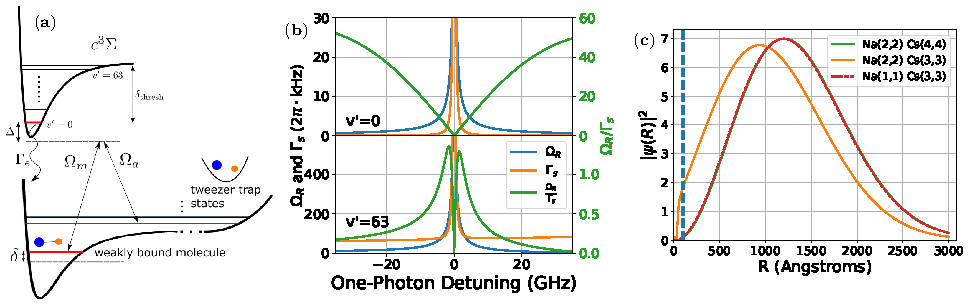
\includegraphics[height=5cm]{fig1.pdf}
  \caption{Optical creation of single molecule from single atoms in tweezer.
    (A) Schematics of the optical transition from an atom pair to a weakly bound molecule.
    The initial state is the relative motional ground state between the two atoms
    and the final state is the first molecular bound state.
    The transition is driven by a pair of laser frequencies matching the binding energy
    of the molecule.
    The lasers are detuned from an excited molecular state in the $c^3\Sigma$ potential
    by $\Delta$ in order to suppress the scattering during the transfer.
    (B) Comparison between using a weakly bound and a deeply bound excited state
    as intermediate state for the Raman transition.
    The deeply bound excited state (upper half $v'=0$) has a smaller Raman Rabi frequency ($\Omega_{Raman}$)
    compared to the weakly bound excited state (lower half $v'=63$) at a given detuning.
    However, the scattering rate ($\Gamma_{scatter}$) is also much lower,
    which results in a larger Raman Rabi frequency to scattering rate ratio.
    (C) Enhancement of short range wavefunction.
    The large scattering length for the $Na(2,2),Cs(3,3)$ state creates an interaction shift
    comparable to the axial trapping frequency.
    This causes a significant change in the relative wavefunction especially at short
    intranuclear distance ($R$).
    Compared to other spin states with weaker interaction,
    the wavefunction at short distance ($R<100\mathrm{\AA}$) is significantly enhanced.
    \label{f-theory}
  }
\end{figure*}





% In this letter, we will present our result on coherent creation of a weakly bond molecule
% using only optical transitions on a broad optical line for the first time.


% The optical transfer scheme we use is shown in figure \todo{}. To drive the atoms from
% We use an optical Raman transition to drive the system from the atomic initial state to a ground electronic molecular state. In order to reduce the size mismatch between the atomic and molecular states, we selected the first bound state for the 3322 spin state \todo{asymtopt to the 3322 threshold?} as our final state. \todo{move selection of intermediate state to intro?}. For similar reason, the natural choice for the intermediate excited molecular state is one with highly excited motional level.However, from our calculation (and experiment?), the smaller level space for high vibrational state and the smaller detuning from the atomic threshold increases the scattering rate of the molecular state which causes a reduced Raman Rabi frequency to decoherence rate ratio and a lower transfer efficiency. Therefore, in our experiment, we selected the v'=0 state as the intermediate state for our Raman transition.

% While optical Raman transfers of atoms to molecules utilizing an electronic excited state have been shown previously, the transfers were incoherent  where the resulting molecules were lost~\cite{Wynar2000,Rom2004}.
% For a given excited intermediate state,
% This can be understood by using a three level model.
% However, we are constrained by the multi-level of molecules.
% A key difference in molecular association via a Raman process compared to Raman transfer between hyperfine states in atoms is that the matrix elements between the ground states and the excited state are greatly unbalanced. In particular, the matrix element between the molecule state and the excited state, $ \Omega_m $ is much larger than the matrix element between the free atom state and the excited state, $ \Omega_a $. To understand the effect of this imbalance, we consider a 3 level model, and ignore the presence of multiple excited states.

% The challenge of optical Raman association of molecules from atoms lies with achieving a high enough Raman Rabi frequency despite the wavefunction size mismatch between the atomic state and the excited molecular state. While pioneering experiments used weakly bound molecular excited states in the Raman transition to increase the Raman Rabi frequency, such choice of state also increases the scattering during the transfer process to render it incoherent, resulting in molecule loss~\cite{Wynar2000,Rom2004}.
% Therefore, finding the largest Raman Rabi frequency to scattering ratio that enables population transfer with minimal loss is the first key task.

The essence of an optical Raman transfer can be illustrated using a three-level system (Fig.~\ref{f-theory}A), where the initial atomic state, the target weakly-bound molecular state are coupled to an intermediate state by two photons, $\Omega_a$ and $\Omega_m$, with one-photon detuning $ \Delta $, and two-photon detuning, $ \delta$.  %(Ultimately, we calculate with contribution of all vibrational states of the excited electronic potential, $c^3\Sigma^+$)
The transfer Raman Rabi Rate, $ \Omega_a\Omega_m / 2\Delta$, is accompanied by a photon scattering rate that is a sum of all coupling sources%,
% $\Gamma_e \Omega^2 / 4\Delta^2 $, where $ \Gamma_e $ is the excited state linewidth
~\cite{Wineland2003}.
Unlike for Raman transitions in atoms, the two coupling matrix elements here are greatly imbalanced %. Since $ \Omega_m $ is generally much larger than $ \Omega_a $
due to the small wavefunction overlap between the atomic state and the intermediate state, %the atomic state and the excited molecular state,
and therefore the scattering is predominantly from the target molecular state. Furthermore, the energy difference between the atomic state and target molecular state is small ($ < 1~\mathrm{GHz} $) compared to the single photon detuning, $ \Delta $, so the target molecular state can scatter off both beams roughly equally. Thus, the scattering is given by $ \Gamma_e \Omega_m^2 / 2\Delta^2$, where $ \Gamma_e $ is the excited state linewidth \footnote{We choose the two beams to have equal power, which gives the highest Raman Rabi rate at a fixed total power. Thus, this results in a simple factor of 2 coming from scattering off 2 beams.}.
The ratio between the Raman Rabi frequency and the scattering rate is therefore $ \Omega_a/\Omega_m \times \Delta/\Gamma_e $. %, depends on the ratio of the two matrix elements and how far detuned the laser is from the transition in units of the linewidth.
To ensure a coherent process, a detuning as large as possible, while maintaining a realistic Raman Rabi frequency, is preferred. %However, the detuning cannot be too large, since that will reduce the Raman Rabi frequency.
With the multiple excited vibrational states present in a molecular potential as intermediate states, the total scattering rate and Raman Rabi rate become a sum over the scattering rates and Raman Rabi rates of the individual intermediate states. Furthermore, for a more complete calculation, we also need to account for the effects of the excited atomic continuum, which is particularly important for the target molecular state. The sum of the squares of the wavefunction overlap between the target weakly-bound molecular state and all the excited molecular intermediate states considered is only about 2\%, suggesting that there is significant matrix element between the target molecular state and the excited atomic continuum. (See SM)

Pioneering experiments used weakly-bound excited states as the intermediate state in the Raman transition to ensure a large Raman Rabi frequency~\cite{Wynar2000,Rom2004}. However, such choice of state suffers from strong scattering of the nearby excited atomic continuum to render it incoherent, resulting in molecule loss. This scattering is  proportional to $1/\delta_{thresh}^2$, where $\delta_{thresh}$ is the detuning from the dissociation threshold, and thus can  be made smaller by detuning away from the dissociation threshold.


% For a weakly bound molecular state, the spacing between states is generally smaller compared to deeply bound states and thus limits the maximum usable detuning and therefore the effectiveness of the scattering reduction by increasing the detuning.
% Furthermore, due to similarity in wavefunction size, the weakly bound molecular ground state and initial atomic state have strong coupling with the atomic excited state which contributes significantly to the total scattering rate. The rate of such a scattering process is proportional to $1/\delta_{thresh}^2$, where $\delta_{thresh}$ is the detuning from the dissociation threshold, and thus can also be made smaller by detuning away from the dissociation threshold.
% (Should we also mention scattering of the atomic initial state too? This should affect the Raman process as well)

To find the optimal intermediate state, we perform a  calculation of the Raman Rabi frequency and scattering rate at different detunings from the atomic threshold taking into account of all states of the $c^3\Sigma^+(\Omega = 1)$ excited molecular state potential~\cite{Grochola2011} and the continuum~\cite{Liu2017}.
As shown in Fig.~\ref{f-theory}B (full result in SM), the ratio of the Raman Rabi rate to scattering rate can be made larger for more deeply bound states compared to weakly bound states at a cost of a smaller Raman Rabi frequency.
As a result, we choose %a deeply bound molecular excited state
the $v'=0$ of $c^3\Sigma^+(\Omega = 1)$ as an intermediate state to drive the Raman transition. %(mention the trend, also v'=12 will work as similarly as v'=0)

% higher Raman Rabi frequency at the same detuning, using a weakly bound intermediate state results in a much higher scattering rate and ultimately a smaller Rabi frequency to scattering rate ratio as compared to deeply bound states. As a result, we use a deeply bound molecular excited state to drive the Raman transition.

% (goes to SM?)

% (mention scattering/lightshift depends on up/down matrix element ratio?)

% In addition to the intermediate state, the choice of the initial and final states are critical for both fundamental and technical reasons.  Thus, a small $ \Omega_m/\Omega_a $ ratio is desired to be able to drive this transition coherently at smaller detunings where the Raman Rabi frequency will be larger. In addition to this fundamental reason, there is also a technical advantage for having a $ \Omega_m/\Omega_a $ ratio to be as small( KW: I think small, but open question whether we should always talk about $\Omega_m/\Omega_a$ or $ \Omega_a/\Omega_m$, KN: maybe $ \Omega_a/\Omega_m$ is better because it sounds more natural that we want to make it large? but either way.) as possible. The position of the resonance depends on the laser power predominantly through the AC Stark shift on the molecular state, $ \Omega_m^2 / 2\Delta $. The ratio of the AC Stark shift to the Raman Rabi frequency is $ \Omega_m / \Omega_a $, Thus, the laser needs to be stabilized to better than the inverse of this ratio, $ \Omega_a/\Omega_m $, to fluctuate by less than a linewidth. This becomes technically easier wh So en $ \Omega_m/\Omega_a $ is smaller.
% (for our choice of states, this mean intensity fluctuation of less than 1\% or 0.1\%. KW: I mentioned this in next paragraph, does it still need to be mentioned here?)

% \textcolor{blue}{Main point here. Small $\Omega_a/\Omega_m$ ratio can be compensated by larger detuning, but Stark shift is problematic.} \textcolor{red}{KW: I agree Stark shift limitation is definitely pretty problematic, but I would also argue that larger detuning may not be able to save the day, because of the many vibrational states in a molecular potential, the lower Raman rabi frequency which results from detuning farther and possibly running into other limitations if you have to do that, such as the background off resonant scattering rate from near threshold states or technical background scattering.} \textcolor{blue}{yes, I agree. I want to layout the structure .... motivate for the better ratio first, than talk about choosing the state.} \textcolor{red}{KW: Okay, got it. Makes sense. }
% In addition to the intermediate state, the choice of the initial and final states is also critical.
In addition to the intermediate state, choosing an initial and a final state for a large $ \Omega_a/\Omega_m $ ratio would allow large Raman Rabi coupling at a given detuning. Furthermore, a larger ratio also relaxes the intensity stability requirement, because this is also the ratio between the Raman Rabi coupling and the AC Stark shift of the molecular state, $ \Omega_m^2 / 2\Delta $ \footnote{There is an additional factor of 2, with both beams at equal power, to account for the Stark shift caused by both beams.}.
% and relax the intensity stability requirement due to the AC Stark shift of the molecular state, $ \Omega_m^2 / 2\Delta $ \footnote{There is an additional factor of 2 to account for the Stark shift caused by both beams.}
% As previously discussed, the ratio of the Raman Rabi rate to the scattering rate is proportional to the $ \Omega_a/\Omega_m $ ratio. The smaller this ratio is, the farther the laser needs to be detuned to achieve the same Raman Rabi rate to scattering rate ratio, which lowers the Raman Rabi rate. In addition to reducing how far the laser needs to be detuned from the transition, a larger $ \Omega_a/\Omega_m$ ratio also relaxes the intensity stability requirement, a key potential technical limitation. The position of the two photon resonance depends on the laser power predominantly through the AC Stark shift on the molecular state, $ \Omega_m^2 / 2\Delta $ \footnote{There is an additional factor of 2 to account for the Stark shift caused by both beams.}. The ratio of the AC Stark shift to the Raman Rabi frequency is $ \Omega_m / \Omega_a $, Thus, the laser intensity needs to be stabilized to better than the inverse of this ratio to fluctuate by less than a linewidth in a coherent process. The ratio, $ \Omega_a/\Omega_m $ can be changed through the choice of initial and final states.
% Because of the large atom and molecule wavefunction mismatch, choosing an initial atomic state that has more amplitude at smaller internuclear distance can increase the coupling $\Omega_a$. \textcolor{blue}{(the two sentences have the same idea.)}
% it can be made larger by increasing the coupling of the atomic state with the excited molecular state.
Due to the small size of the intermediate state wavefunction, the coupling $\Omega_a$ is approximately proportional to the value of the relative atomic wavefunction at short distance within the molecular potential. To increase the amplitude within the molecular potential, one can increase the external confinement of atom pairs. Using a harmonic oscillator approximation, the short range amplitude is proportional to $ \omega_{\text{trap}}^{3/4} $, where $ \omega_{\text{trap}} $ is the trap frequency. Alternatively, one can choose an atomic pair state with a large scattering length (positive or negative).
For these states, the phase shift in the relative wavefunction between the atoms can significantly increase the short range wavefunction (Fig.~\ref{f-theory}C). %The increase in the coupling is proportional to (quote/cite Olive's equation?).
For our system of Na and Cs atoms, we choose  a spin state combination $\ket{\uparrow_{\text{Na}} \downarrow_{\text{Cs}}}\equiv \ket{F=2,m_F=2}_{\text{Na}}\ket{F=3,m_F=3}_{\text{Cs}} $that has a large and negative scattering length of $ a(\uparrow_{\text{Na}} \downarrow_{\text{Cs}}) = -693.8a_0$~\cite{Hood2019}. We note that other stable spin combinations give smaller scattering lengths ($<~50~a_0$).
% We denote the possible hyperfine states of the atoms as $ \ket{\uparrow_{\text{Cs}}} = \ket{F=4,m_F=4}_{\text{Cs}}, \ket{\downarrow_{\text{Cs}}} = \ket{F=3,m_F=3}_{\text{Cs}}, \ket{\uparrow_{\text{Na}}} = \ket{F=2,m_F=2}_{\text{Na}}, $ and $ \ket{\downarrow_{\text{Na}}} = \ket{F=1,m_F=1}_{\text{Na}}$. Among the stable spin combinations, $\ket{\uparrow_{\text{Na}}\uparrow_{\text{Cs}}}$ and $\ket{\downarrow_{\text{Na}}\downarrow_{\text{Cs}}} $ both have small scattering lengths of $ 30.4a_0 $, and $ 13.7a_0 $ respectively, but the $\ket{\uparrow_{\text{Na}} \downarrow_{\text{Cs}}} $ combination has a large and negative scattering length of $ a(\uparrow_{\text{Na}} \downarrow_{\text{Cs}}) = -693.8a_0 $ (interaction shift $\approx$ binding?)~\cite{Hood2019}.
In addition to the increased atomic coupling, $ \Omega_a $, %with the $\ket{\uparrow_{\text{Na}} \downarrow_{\text{Cs}}}$ hyperfine combination,
coupled channel calculations show that the target molecular state that is predominantly in this spin combination also has reduced coupling, $ \Omega_m $, with the intermediate state when compared to bound states of the other stable spin combinations % $\ket{\uparrow_{\text{Na}}\uparrow_{\text{Cs}}}$ and $\ket{\downarrow_{\text{Na}}\downarrow_{\text{Cs}}} $ bound states.
Therefore, using an initial $\ket{\uparrow_{\text{Na}} \downarrow_{\text{Cs}}}$ hyperfine combination results in a $ \Omega_a/\Omega_m$ ratio of about 0.05 instead of a ratio of about 0.003 with the other combinations, and thus only an required intensity stability of 5\% instead of 0.3\%.
% Thus, instead of a required intensity stability of $0.3 \% $ for the 4422 or 3311 combination, the 3322 combination only requires the intensity to be stabilized to $ 5\% $.
% Thus, we choose the $\ket{\uparrow_{\text{Na}} \downarrow_{\text{Cs}}}$ spin combination as our initial state and drive to the first bound state for the $\ket{\uparrow_{\text{Na}} \downarrow_{\text{Cs}}}$ spin combination.
\textcolor{blue}{(clean up the paragraph some more).} %(We might want to mention that those ratios are for 80 kHz spherical trap if we want to give more details about the coupled channel calculation anywhere...)

% In additional to the final and the excited state, it is also important to select the an initial atomic state in order to improve the coupling.
\begin{figure*}[ht!]
  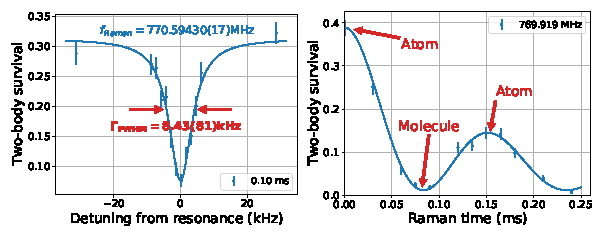
\includegraphics[height=4.5cm]{fig2.pdf}
  \caption{
    (A) Geometry and polarization of trap and Raman beam relative to the bias magnetic field.
    The tweezer and Raman beam is focused through an objective to define the location of the
    atoms and molecule.
    We use a bias B field of $B_0=8.8 G$ alone the tweezer polarization
    to define the quantization axis.
    As a result, the atoms experiences predominately $\pi$ polarization from the tweezer.
    (B) Molecule formation pulse sequence. The tweezer initially consists of only up leg power.
    When driving the Raman transition, the up leg power is smoothly ramped down and
    the down leg power ramped up over $10\mu s$ while maintaining the total power of the tweezer.
    This minimizes the heating on the atoms due to power fluctuation while maximizes the time
    with maximum Raman Rabi frequency when the up and down leg powers are equal.
    (C) Raman resonance from atomic state $Na(2,2)\ Cs(3,3)$ to the first molecular bound state
    using a $0.12\mathrm{ms}$ pulse.
    The full width half maximum (FWHM) of $7.56(82) \mathrm{kHz}$ of the resonance
    is consistent with the FWHM for a coherent $0.12\mathrm{ms}$ $\pi$ pulse $6.7 \mathrm{kHz}$.
    (D) Raman pulse time scan on resonance. A decaying Rabi oscillation can be observed
    proving the coherence of the Raman transfer process.
    \label{f-raman}}
\end{figure*}




%% Preparation
Experimentally, we first prepare two atoms in a well-defined external and internal quantum state using techniques developed previously~\cite{Liu2018, Liu2019, Wang2019}. In brief, the experimental cycle begins by  loading a single ${}^{23}\mathrm{Na}$ atom and a single ${}^{133}\mathrm{Cs}$ atom stochastically into separate optical tweezers. The atoms are initially imaged to distinguish between loading of two atoms, one atom (Na or Cs), or no atom, which is compared to the image at the end of the experiment. Raman sideband cooling is then applied to cool both atoms simultaneous into the 3-dimensional motional ground state of their optical tweezers. After cooling, the Na and Cs atoms are in a spin state of $\ket{\uparrow_{\text{Na}}\uparrow_{\text{Cs}}}\equiv \ket{F=2,m_F=2}_{\text{Na}}\ket{F=4,m_F=4}_{\text{Cs}} $ %and are merged into the same tweezer~\cite{Liu2019}. %The spin states for the Na and Cs atoms after RSC and during the merge process are $\ket{\uparrow_{\text{Na}}\uparrow_{\text{Cs}}} $.
that has a low scattering length. The small two atom interaction allows the two atoms to be merged into the same tweezer with minimum pertubation and remain in the motional ground state after the merge.

% After preparing the Na and Cs atoms in the same tweezer in a single quantum state,
Next, we  drive the atoms into the large scattering length $\ket{\uparrow_{\text{Na}} \downarrow_{\text{Cs}}}$ hyperfine combination as the initial atomic state of Raman transfer by performing a Cs spin flip while taking into account the $-30.7 kHz$ interaction shift~\cite{Hood2019}.  %using a Cs Raman transition to drive the Cs atom into the $\ket{\downarrow_{\text{Cs}}}$ state. The new spin state combination has a larger scattering length of $-693.8 a_0$ which generates a interaction shift of $-30.7 kHz$ in the tweezer.
This spin flip selectively transfers atoms in the relative motion ground state \footnote{This interaction shift is larger than the differential axial trapping frequency between Na and Cs atoms, which decouples the relative and center of mass motional state and improves the robustness of our preparation of the relative motion ground state.}, and for the experiment reported here, this is 31\% of the initial population of two atoms loaded in separate optical tweezers.
% The stronger interaction in this spin state also enhances the atomic wavefunction at short range and increases its overlap with the intermediate molecular state used for our Raman transfer..

%% Transfer scheme
% After the atoms are prepared in the $\ket{\uparrow_{\text{Na}}\uparrow_{\text{Cs}}} $ hyperfine combination, we then perform the Raman transfer.
To perform Raman transfer of an atom pair to the target weakly-bound molecular state, we use the tweezer itself as the Raman beams by turning on two co-propagating frequencies in the tweezer during the Raman pulse (Fig.~\ref{f-raman}A). The dual use of the tweezer beam not only eliminates additional scattering sources or undesired laser frequencies, but also allows a tight focus to maximize the Raman Rabi frequency and minimize the transfer time. %to allow perfect overlap and to eliminate additional beams and therefore scattering sources.
The pulse sequence is shown in Fig.~\ref{f-raman}B. %Instead of adding another beam to drive the Raman transition on the atoms in the tweezer, we use the tweezer itself to achieve this goal.
% In particular, we turn on two co-propagating frequencies in the tweezer during the Raman pulse. The dual use of the tweezer beam ensures that there is not any undesired laser frequency that can interfere with the Raman transition, and also allows us to maximize the Raman Rabi frequency and minimize the transfer time.
After the total tweezer power is set to the desired value, we smoothly ramp down the power of one frequency in the tweezer while simultaneously ramping up the power of a different frequency so that the total tweezer power remains unchanged. Both frequencies are kept on for a specified duration before the process is reversed and the tweezer returns to a single frequency.
% In addition to reducing the number of laser beams during the Raman transition,
Furthermore, we use a Bragg grating with a linewidth (FWHM) of $50 ~\mathrm{GHz}$ to filter the laser spectrum generated by a fiber amplifier that is seeded with a $1037~\mathrm{nm}$ external cavity diode laser. We observed a reduction of the scattering rate by a factor of $2$ due to suppression of the broadband amplified spontaneous emission (ASE) from the laser that couples to other excited states.

% found the spectral purity of the laser for Raman beams to be critical for achieving a higher transfer efficiency.
% The tweezer/Raman beams are generated by a fiber amplifier seeded with a $1037 \mathrm{nm}$ external cavity diode laser.
% by amplifying a $1037 \mathrm{nm}$ external cavity diode laser (ECDL) with a fiber amplifier,
% The diode laser produces the desired frequency on top of a broad band amplified spontaneous emission (ASE).  We use a Bragg grating with a line width (FWHM) of $50 \mathrm{GHz}$ to clean up the laser spectrum and found it reduces the scattering rate by at least a factor of $2$
% for a particular single photon detuning.

% in addition to the desired frequency. This increases the scattering rate due to coupling to other excited states.

\begin{figure*}[t!]
  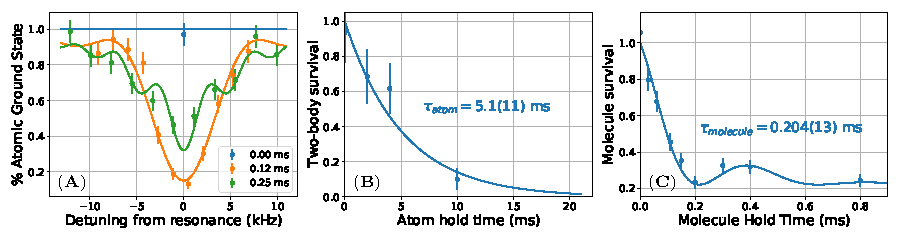
\includegraphics[height=4.5cm]{fig3.pdf}
  \caption{
    (A) Fitting of Raman detuning scans at different times to a model of Raman transition
    with loss on the atom and molecule state. The combined fit is used to determine
    both the Raman Rabi frequency and the loss rates.
    (B) \todo{inset?} Two-body atom lifetime in $15 \mathrm{mW}$ of trap depth caused by
    off-resonance photoassociation.
    This is used to improve the fitting of the Raman transfer data.
    (C) Direct measurement of molecule lifetime in $15 \mathrm{mW}$ of trap depth.
    Molecule survival is detected by dissociating back to atoms using a second Raman transition.
    The lifetime is consistent with the $0.204(13) \mathrm{ms}$
    measured from the Raman transition data.
    The oscillation in the survival is the result of the interference
    between the two Raman pulses with incomplete transfer.
    \label{f-lifetime}}
\end{figure*}

%% Experiment condition/resonance

Guided by coupled channel calculations, we locate the Raman resonance for the atom to molecule transition at $770.59430(17) ~\mathrm{MHz}$ (Fig.~\ref{f-raman}C) with a $15 ~\mathrm{mW}$ tweezer at $288560 ~\mathrm{GHz}$ which corresponds to a $145 ~\mathrm{GHz}$ single photon detuning.
% (We can maybe add information about the prediction here?)
%% Prediction
% This excited state used in the Raman transition was measured in our previous experiment using photoassociation to be at $288560 GHz$ from our atomic state. The ground molecular state has not been observed previously in experimentally. Based on our measurement of FB resonance, interaction shift and the binding energy of the 4422 bound state. Theory prediction was at $770.1 MHz$. \todo{more, mention/cite Jeremy}
% The background level of $31\%$ corresponds to the probability of preparing the two atoms in the relative motional ground state.
% When the atoms are transferred into the molecule state by the Raman transition, there is a decrease in the two body survival since the resulting molecule is dark to our imaging sequence. % directly detected by our imaging step.
The molecular state is dark to the imaging step, so successful transfer of the atoms to the molecular state will be detected as loss of atoms in the post experiment image when compared to the initial image. We observed the narrowest linewidth of $7.56(82) \mathrm{kHz}$ for the Raman resonance at a pulse time of $0.12 \mathrm{ms}$, which corresponds to a linewidth-pulsetime product of $0.907(98)$. This is consistent with the expected value of $0.80$ for an ideal $\pi$ pulse which is evidence of a coherent transfer. In order to verify the coherence of the transfer directly, we fix the two photon detuning on resonance and scan the pulse time. Fig.~\ref{f-raman}D shows the observed Rabi oscillation between the atomic and molecular states. Fitting the data with a decaying Rabi oscillation suggests that $69\%$ of initial ground state atoms are transferred into the molecular state.

In order to understand the fidelity of molecule formation, we fit our measurements to a model that includes a Raman Rabi frequency and a finite lifetime for the molecular state (Fig.~\ref{f-lifetime}A). We account for the effect of atomic state loss by measuring the single and two body lifetime of the atoms directly (Fig.~\ref{f-lifetime}B) without turning on the second frequency. The fit shows that we have a Raman Rabi frequency of $2\pi\times3.282(42) ~\mathrm{kHz}$. The molecule we form has a lifetime of $0.204(13) ~\mathrm{ms}$ which is the main limitation on the fidelity of the transfer. The molecule lifetime can be measured directly by preparing the molecule with a $\pi $ pulse and then using a second $\pi $ pulse to dissociate the molecule back to atoms after a variable wait time (Fig.~\ref{f-lifetime}C). The result shows a molecular lifetime consistent with our fitting of the decaying Rabi oscillation.

The ratio of the molecule scattering rate to the Rabi frequency is larger than
the theory prediction by more than a factor of $10$.
Based on the discussion above, if this discrepancy arises from the $v'=0$ excited state,
it can be either due to a high ratio of $\Omega_m / \Omega_a$ or a large $\Gamma_e$.
Additionally, coupling to other excited states can also add an offset to
both the Raman Rabi frequency and the scattering rate
which can affect the scattering rate to Rabi frequency ratio.

In order to verify whether any one of these known sources are the origin of the discrepancy,
we measured the Raman resonance as a function of the tweezer power and single photon frequency.
These dependencies allow us to experimentally determine the matrix elements,
$ \Omega_a $, $\Omega_m $ and how much of the scattering, Stark shift,
or Raman Rabi frequency comes from the $ v' = 0$ intermediate state.

First we look at the change in resonance frequency.
As a function of the tweezer power,
we observe the expected linear dependency on the resonance frequency
caused by the differential light shift between the atomic and molecular state (Fig.~\ref{f-det}A).
When we vary the tweezer frequency around the $v'=0$ intermediate state,
we can further observe a $1/\Delta$ component
and a constant background in the experimentally explored region.
The background is caused by coupling to other excited states that are further away in energy.
The $1/\Delta$ component, however, is due to the coupling between the molecular state
and the $v'=0$ intermediate state.
From this measurement, we can calculate a $\Omega_m$ of
$2\pi\times36.162(20) ~\mathrm{MHz}/\sqrt{\mathrm{mW}}$ or
$2\pi\times140.056(78) ~\mathrm{MHz}$ for the $15 ~\mathrm{mW}$ tweezer power used above.
This number is consistent with the value of
$2\pi\times27 \mathrm{MHz}/\sqrt{\mathrm{mW}}$ calculated from theory. \todo{ref/sm theory}

\begin{figure*}
  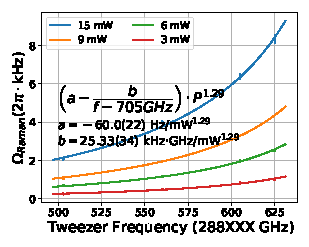
\includegraphics[height=4.5cm]{fig4.pdf}
  \caption{Raman transition parameters as a function of tweezer and Raman power and detuning.
    (A) The light shift of the Raman resonance scales as $P_{tweezer}$
    and follows $1/\Delta$ with an offset.
    The fit also includes a small term that is proportional to $P_{tweezer}^2$
    which is caused by the effective magnetic field generated by the tweezer which is
    perpendicular to the real magnetic field.
    (B) Raman Rabi frequency scales as $P_{tweezer}^{1.29}$ and follows $1/\Delta$ with an offset.
    From these results we can confirm the theory prediction of
    the atom-molecule matrix element ratio.
    (C) Atomic scattering rate scales as $P_{tweezer}^{2.58}$,
    this is consistent with a two photon scattering process.
    We have not measured a clear dependency of the loss rate on the tweezer detuning.
    \label{f-det}}
\end{figure*}

In order to calculate the matrix element ratio,
we now need to extract the matrix element, $ \Omega_a $.
We do this by measuring the dependencies of the Raman Rabi frequency,
which depends on both $\Omega_m$ and $\Omega_a$.
The Raman Rabi frequency shows a non-linear dependency on the tweezer power
due to the change in the atomic wavefunction caused by
tighter confinement at higher power (Fig.~\ref{f-det}B).
Thus, as discussed before, for weakly interacting particles,
$\Omega_a$ scales as $ \omega_{\text{trap}}^{3/4}$ or $P^{0.375}$.
However, due to the strong interaction between the two atoms, this approximation breaks down.
Instead, coupled-channel calculation shows that the scaling
is very well approximated by $P^{0.29}$ within the range of confinement in our experiment.
Combined with the standard intensity factor, the Raman Rabi frequency should scale as $P^{1.29}$,
which agrees with our experimental result.
Similar to the light shift, there is also a constant background component
and a $v'=0$ component in the Raman Rabi frequency that scales as $1/\Delta$.
The $v'=0$ component of the Raman Rabi frequency is
$2\pi\times161.8(22) ~\mathrm{Hz\cdot mW^{-1.29}}$,
or $2\pi \times 5.324(73)~\mathrm{kHz}$ at $15 ~\mathrm{mW}$ tweezer power.
Together with the $\Omega_m$ measured above, the up leg Rabi frequency is
$2\pi \times 11.53(16)\mathrm{MHz}$.
This gives a Rabi frequency, and therefore matrix element, ratio of $12.14(16)$,
which is in fact better than the theory prediction of $23.7$
and should not cause the ratio of the Raman Rabi frequency to scattering rate
from the $v'=0$ state to be higher than expected.
Furthermore, based on measurements of the excited state using photoassociation (PA) spectroscopy,
the natural linewidth of the $v'=0$ excited state is no larger than $20 \mathrm{MHz}$.
This suggests that the excited state linewidth should not cause
a stronger than expected scattering from $v'=0$ state either.

With the $ v' = 0 $ state ruled out as the source of discrepancy between experiment and theory,
we now consider the background effects from other states with larger single photon detuning.
Unfortunately, the background in the Raman Rabi frequency fit cancels the Rabi frequency
for a single photon detuning that is red of the $ v' = 0 $
and reduces it by about $30\%$ at the current detuning.
However, this difference is not enough to explain the over factor of $10$ discrepancy
present in the experiment.
The same offset will increase the Rabi frequency for blue detuning,
but we have observed additional excited states at slightly higher frequencies
which prevent the blue side of the transition to be usable for the Raman transition.

\todo{change scattering to decoherence? since the fluctuation of light shift
  does not lead to scattering but only decherence.}
These results suggest that the decoherence or loss we observed during the Raman transition
comes from either a higher than expected background scattering rate
or a different intrinsic or technical source that we have not accounted for.
We have observed a significant decrease in the coherence time without the ASE filter,
suggesting the spectral purity of the laser is a significant source of scattering.
Another source of decoherence could result from fluctuations in the power ratio
between the two beams resulting in a fluctuation in the resonance position.
In the experiment, we only stabilize the total power of the tweezer.

In additional to calibrating the $\Omega_m$ and $\Omega_a$,
the scattering rate of the molecule is also depend on the tweezer power and detuning.
At $3\mathrm{mW}$ tweezer power, we have observed molecule lifetime as long as $1\mathrm{ms}$.
However, since the technical noise that can lead to decoherence
is not fully characterized in our experiment,
we are unable to further identify the source of the discrepancy based on this dependency.

Lastly, to confirm that the excess scattering does not come from the atomic state,
we measure the two-body scattering rate
without turning on the second frequency (Fig.~\ref{f-det}C).
The scattering rate scales as $P_{tweezer}^{2.58}$ which is inconsistent
with a single photon scattering process.
We have not been able to observe a dependency on the detuning in order to verify
if the scattering process is related to the $v'=0$ state,
but the power scaling strongly suggests the existence of a unknown two photon scattering process.
Nevertheless, the absolute scattering rate is much lower than the total scattering rate
and is not the limiting factor in our experiment.

%%%% Maybe this following section about the B field can be relegated to a figure caption?
% Figure () shows the geometry of the experiment setup. A $8.8\mathrm{G}$ B field was used to defines the quantization axis in the experiment and is applied perpendicular to the tweezer axis. The tweezer beam (both frequencies for the Raman transition) has a $\pi$ polarization relative to the quantization axis, which allows us to selectively drive the Raman transition to a final state with the same total $m_F$ quantum number as our initial state.
B field dependency $42.17(24) kHz/G$.

In conclusion, we have formed a weakly bound NaCs molecule in an optical tweezer via an optical Raman transfer. A theoretical investigation including all excited states of $ c^3\Sigma^+(\Omega = 1)$, the excited atomic continuum and coupled channel ground state wavefunctions indicated better transfer efficiency using a deeply bound intermediate state and the $ \ket{\uparrow_{\text{Na}} \downarrow_{\text{Cs}} } $ hyperfine state combination. Using these theoretical insights, we located the weakly bound state and coherently associated the atoms into the weakly bound molecule. Our transfer efficiency is limited by an unknown scattering source resulting in measured scattering rates over 10 times larger than theory predictions. Despite this limitation, the transfer efficiency may be further improved by increasing the $ \Omega_a/\Omega_m$ ratio by exploring the possibility of driving to more deeply bound states. There may also be a better choice of single photon detuning to increase the Raman Rabi frequency, since our location results in about 30\% cancellation of the Raman Rabi frequency due to an offset of unknown origin. Nevertheless, our technique, with the right choice of parameters, can be used to form a more diverse set of molecular species, since it does not rely on a magnetic Feshbach resonance, bound states at the MHz-level or a narrow excited state. The formation of a weakly bound molecule is a key step in forming rovibrational ground state molecules. Combined with real time rearrangement \cite{Barredo2016, Endres2016}, defect free arrays of highly controlled molecules can be formed in arbitrary geometries. These arrays are a promising and flexible platform for quantum simulation and quantum computing applications.

\todo{sm: STIRAP vs Raman}

\begin{acknowledgments}
  We would like to thank Bo Gao and Paul Julienne, Rosario (?) (anybody else) for discussion. This work is supported by the NSF~(PHY-1806595), the AFOSR~(FA9550-19-1-0089), ARO DURIP (W911NF1810194) and the Arnold and Mabel Beckman foundation. J.~T.~Z. is supported by a National Defense Science and Engineering Graduate Fellowship. W.~C. is supported by a Max Planck-Harvard Research Center for Quantum Optics fellowship. K.~W. is supported by an NSF GRFP fellowship. J.~M.~H. is supported by the U.K. Engineering and Physical Sciences Research Council (EPSRC) Grants No.\ EP/N007085/1, EP/P008275/1 and EP/P01058X/1.
\end{acknowledgments}

\bibliography{master_ref}
\bibliographystyle{apsrev4-2}
\end{document}

% Fig2 make vertical remove 2C
% Bigger dots
